\documentclass[15pt, onecolumn]{article}
% \documentclass[12pt, onecolumn]{article}
\usepackage[utf8]{inputenc}
\usepackage{graphicx}
\graphicspath{ {images/} }
\usepackage{caption}
\usepackage{subcaption}
\usepackage{lipsum}
\usepackage{float}
\usepackage{pdfpages}
\usepackage{hyperref}
% You can set the margine of the text by setting the top, bottom, left and right properties. Also, if using more than one columns, you can change the columnsep property to set the seperation space between two columns.
\usepackage{listings}
\usepackage[a4paper,top=30mm,bottom=30mm,columnsep=6mm,left=20mm,right=20mm]{geometry}
\usepackage{xcolor}
\hypersetup{
    colorlinks,
    linkcolor={red!50!black},
    citecolor={blue!50!black},
    urlcolor={blue!80!black}
}
% uncommnet and change the following two commands to set seperation line width between coulmns.

% \setlength{\columnsep}{1cm}
% \setlength{\columnseprule}{0.6pt}

%########################## Paper Meta data#########################
% You can change the variables in the following section to set them globally thrghout the whole paper.

% Title of the paper
\newcommand{\papertitle}{CO LAB 7 REPORT}
\newcommand{\shorttitle}{PIPELINING IN VERILOG}

% Full name of the author(s)
\newcommand{\authorname}{Neeraj Krishna N (112101033)\\ Amithabh A (112101004)\\Evans Samuel Biju (112101017)}

% Module code
\newcommand{\acmodulecode}{CS2160}

% Module name
\newcommand{\acmodulename}{Computer Organisation Laboratory}

% Name of the college
\newcommand{\accollegename}{Computer Science And Engineering}

% Date
\newcommand{\wrdate}{2 May 2023}
%########################## Paper Meta data#########################

\usepackage{fancyhdr}
\pagestyle{fancy}
\fancyhead{}
\fancyhead[L]{\textsc{\shorttitle}}
\fancyfoot{}
\fancyfoot[R]{\thepage}
\fancyfoot[L]{\acmodulecode\  \textsc{\acmodulename}}
% \fancyfoot[C]{\thepage}
\renewcommand{\headrulewidth}{0.6pt}
\renewcommand{\footrulewidth}{0.6pt}


\title{\papertitle}
\author{\authorname}

\begin{document}
\begin{titlepage}
  \begin{center}
      \vspace*{1cm}

      
\includegraphics[width=\textwidth]{images/IIT_PALAKKAD_LOGO.png}
      
      % \vspace*{1cm}
      \vfill

      \Huge
      % \textsc{Literature Review}
      
      % \vspace{0.5cm}
      
      % \LARGE
      \textbf{\papertitle}
      
      % \vspace{1.5cm}
      \vfill
      
      \Large
      Submitted By\\
      \textbf{\authorname}

      \vspace{1.5cm}

      \large
      \acmodulecode\ \textsc{\acmodulename}
      
      \vspace{0.7cm}
      
      \large
      \textsc{\accollegename}
      
      \vspace{0.7cm}
      
      \Large
      \wrdate
      
  \end{center}
\end{titlepage}
{
  \hypersetup{linkcolor=black}
  \tableofcontents
}
% {
%   \hypersetup{hidelinks}
%   \tableofcontents
% }
% \tableofcontents
\clearpage

\section{Problem Statement of Lab 7}
% This part of the paper discusses the introduction to the subject \cite{Dummy1}.

% \begin{figure*}[h]
%     \centering
%     \includegraphics[width=0.4\linewidth]{dummy}
%     \caption{Dummy figure with citation \cite{Dummy1}.}
%     \label{fig1:dummy}
% \end{figure*}

% \lipsum[1-3]
% This is the complete report of the pipeline which we have done using Vivado
% \subsection{Problem Statement of Lab 7}
We have to add instruction cache (I-Cache) and data cache (D-Cache) to our existing RISV-V datapath RTL. Both I-Cache and D-Cache should be able to store a minimum of eight 32-bit data.
\begin{figure}[h]
    \centering
    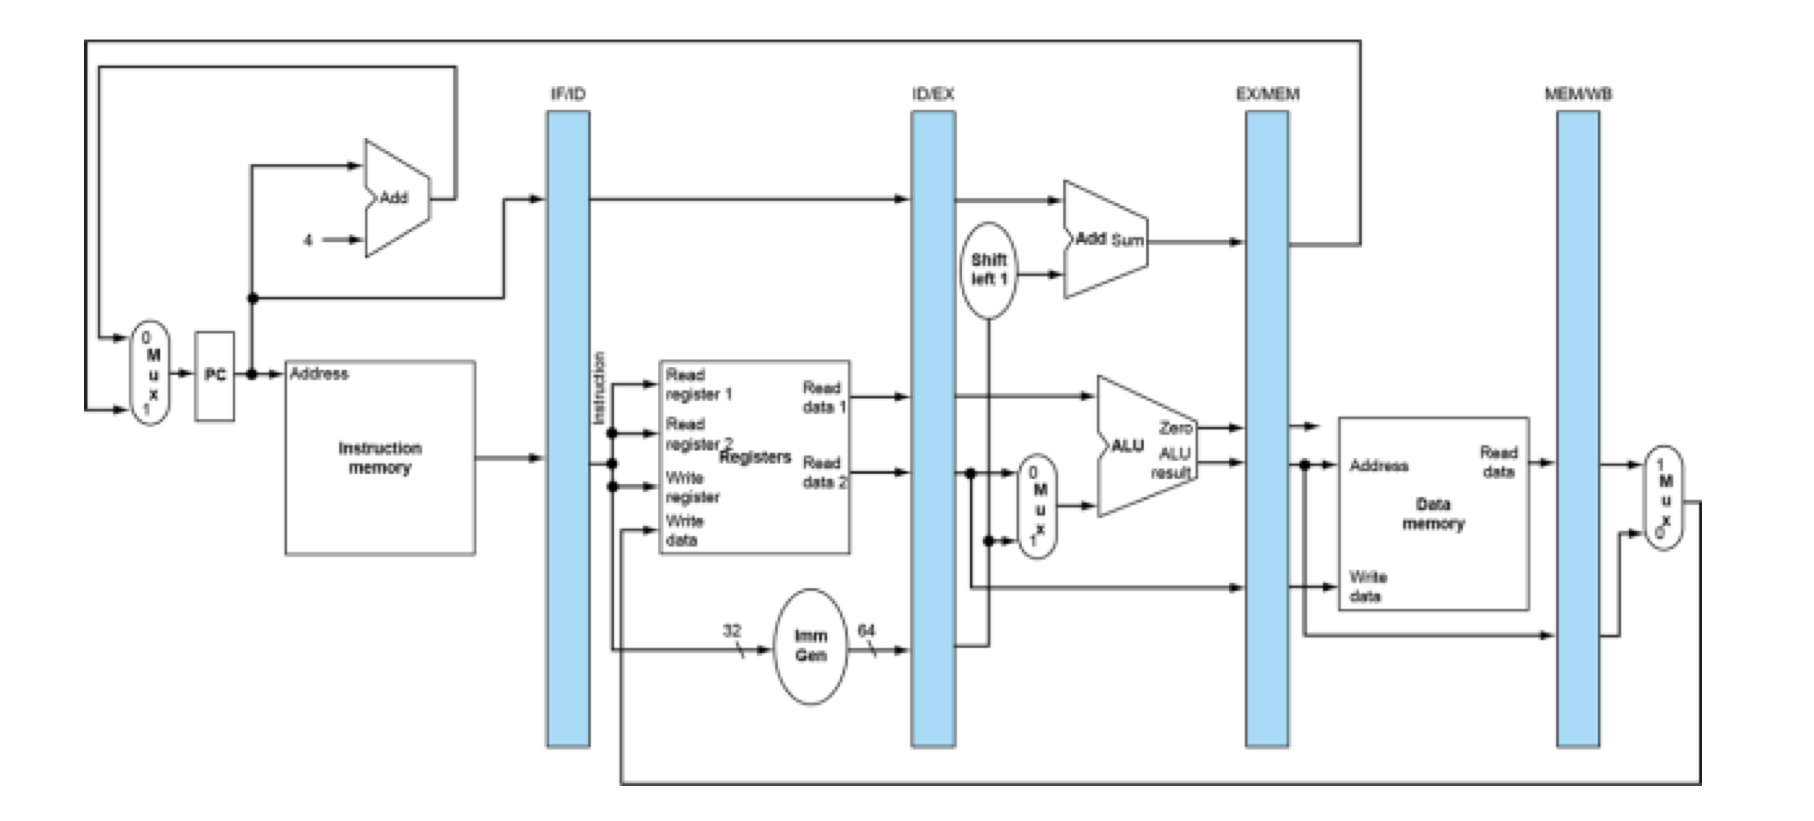
\includegraphics[width=\linewidth]{images/datapath_lab_7.jpeg}
    \caption{RISC-V Datapath}
    \label{fig1:lab_datapath}
\end{figure}

We have to store the following instructions in I-Cache.
\begin{table}[h]
\centering
\begin{tabular}{|c|c|}
\hline
\textbf{Address} & \textbf{Instruction} \\ \hline
000              & addi x29, x29, 0     \\ \hline
001              & addi x30, x30, 1     \\ \hline
010              & lw x28 0(x29)        \\ \hline
011              & lw x27 0(x30)        \\ \hline
100              & add x10, x28, x29    \\ \hline
101              & sw x10, 0(x29)       \\ \hline
\end{tabular}
\caption{Instructions}
\label{given_instructions}
\end{table}
We can store 45 and -20 in the D-Cache initially.

\section{Solution}
Here since we need to add D-Cache and I-Cache, in the existing pipline module we would have to add an 8-length array of 32-bit registers for D-Cache and the instruction is received as an input to the pipeline module.
% \\[0.2in]
% \makebox[\textwidth]{hello}
% \begin{lstlisting}
%   import numpy as np
% \end{lstlisting}
% \begin{lstlisting}[label=some-code,caption=Some Code]
%   public void here() {
%       goes().the().code()
%   }
%   \end{lstlisting}
  
% \lstset{language=Java}
% \begin{lstlisting}
%   public class void main(String args){
    
%   }
% \end{lstlisting}

% the below is the template
% \lstset{language=Verilog}
% \begin{lstlisting}
%   module alu_with_clk(
%     input A,B
%   );
%   endmodule;
% \end{lstlisting}

The complete code for the pipeline can be found in the \href{https://github.com/nnk03/PIPELINE-GROUP-13-BATCH-2021-CO-LAB-IIT-PALAKKAD}{GITHUB REPO}

The code for pipeline and testbench is in the final section of this report \ref{code_section}.
\\
The pipeline receives the instruction as a 256 bit string. The pipeline has an instruction cache which is 8-length array of registers of 32-bit instruction named \textbf{instruction\textunderscore cache}.
For the data cache, it is also an 8-length array (named \textbf{data\textunderscore
cache}) of registers which can hold 32-bit values which is declared inside the pipeline module. When \textbf{rst is 1}, all the values inside the register file resets to zero and the \textbf{instruction\textunderscore cache} inside the pipeline module will have the correct instruction in the correct addresses. And, the whenever posedge clk happens, the pipeline which is modelled as an FSM will go from \textit{STAGE 1} to \textit{STAGE 4} at each posedge clk. \textbf{Instruction Fetch} happens when the current stage is \textit{STAGE 1}.
The type of instruction (i.e. whether it is load instruction, store instruction, or R-Type instruction or I-Type instruction) is obtained from the decoder. 
The schematic for the design is shown before the section "Code for Lab 7"$^{\ref{code_section}}$ .i.e. here \ref{schematic} (The schematic is in landscape view).

\begin{itemize}
  \item When it is a load instruction, say for example \textit{lw x28, 0(x29)}, it takes the value of \textit{x29}, adds the offset 0 and stores the value in this address of the \textbf{data\textunderscore cache} to \textit{x28}.
  \item When it is a store instruction, say for example \textit{sw x28, 0(x29)}, it stores the value in the register \textit{x28} to the \textbf{data\textunderscore cache} at the address \textit{x28} added with the offset 0.
  \item When it is an R-Type instruction, say for example, \textit{add x29, x28, x28}, it takes the value of \textit{x28} and adds it with itself and writes it to the register \textit{x29}.
  \item When it is an I-Type instruction, say for example, \textit{add x29, x28, 5}, it takes the value of \textit{x28} and adds it to \textit{5} and writes it to the register \textit{x29}.

\end{itemize}

% 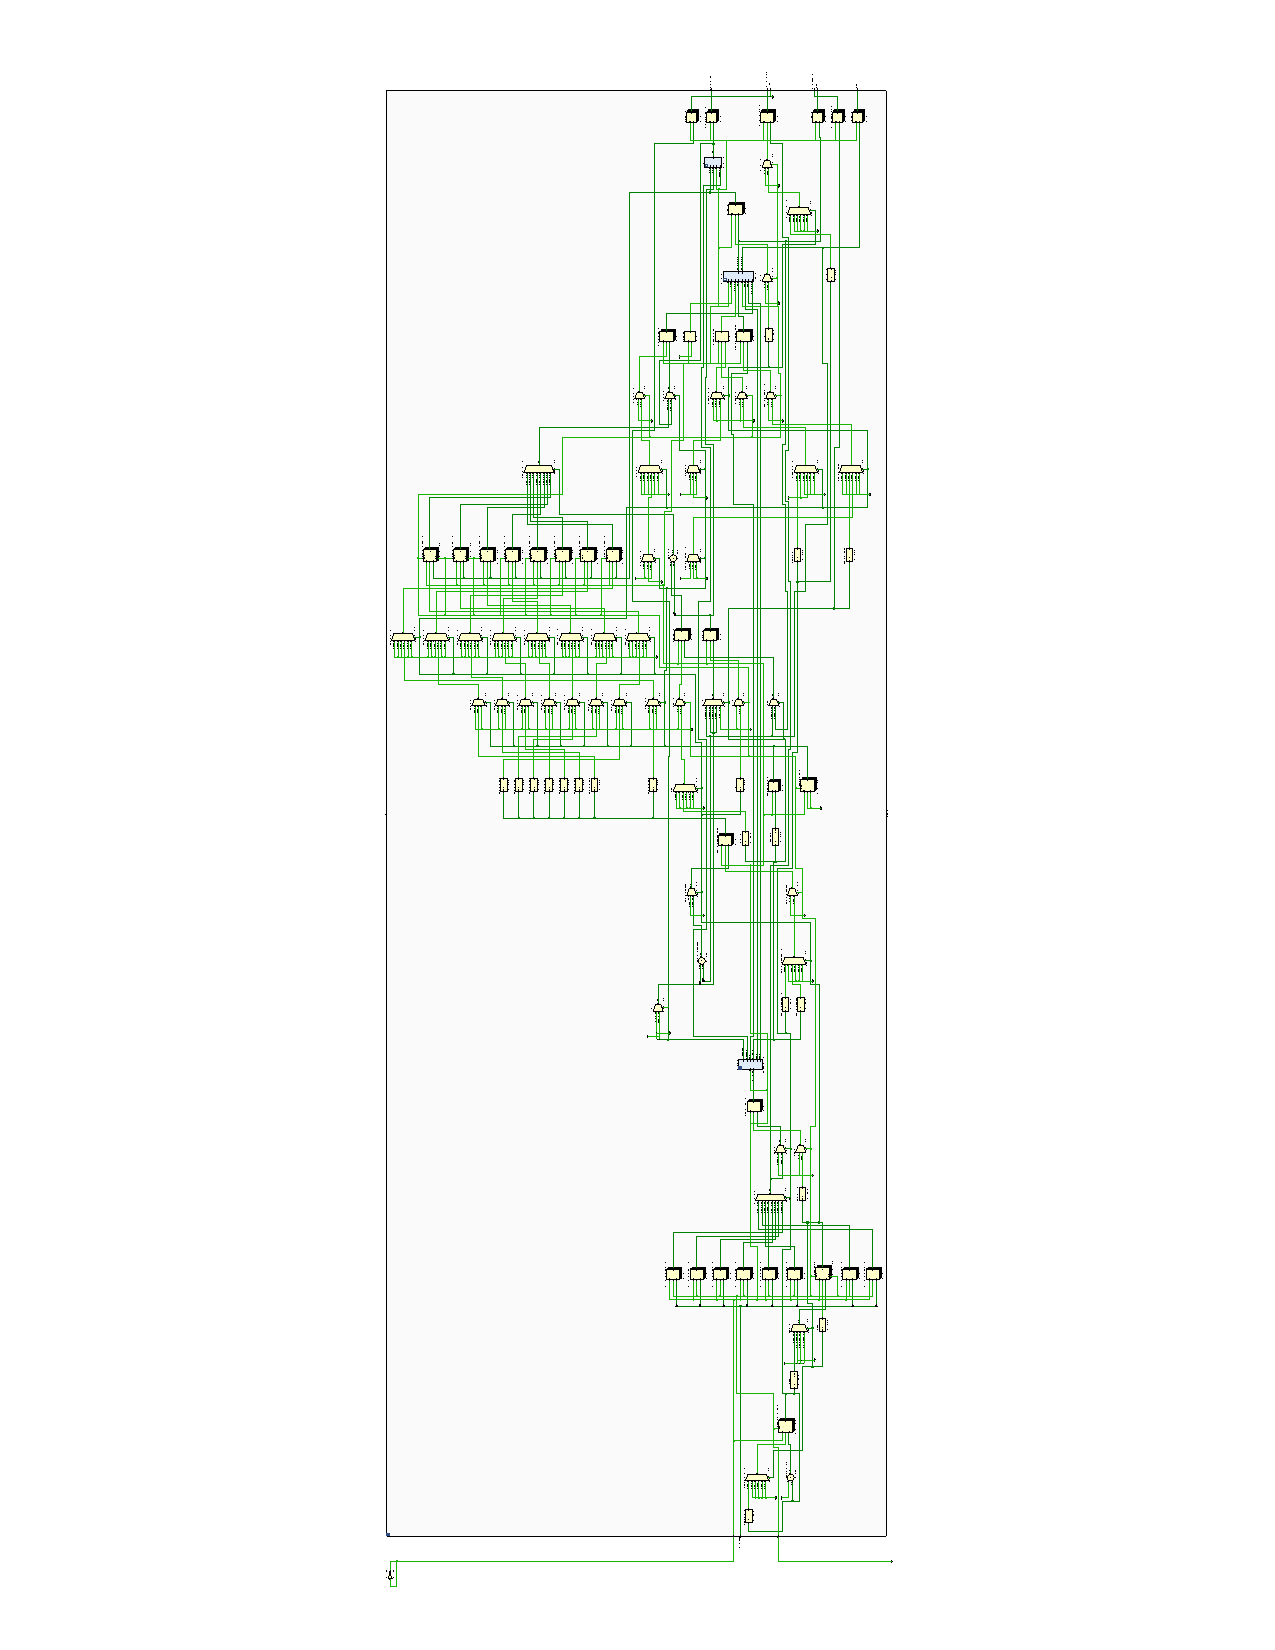
\includepdf[page={1}]{PIPELINE_LAB_7_SCHEMATIC_LANDSCAPE}


% \clearpage
% \section{Related Work}
In this section you can mention the recent studies around the subject of the paper 
% \cite{Dummy2}\cite{Dummy3}.

% \lipsum[5-10]
\section{Timing Diagrams}
The timing diagram for the testbench is shown in Figure$^{\ref{simulation_image}}$

% \lipsum[1-5]
\begin{figure}[H]
  \centering
  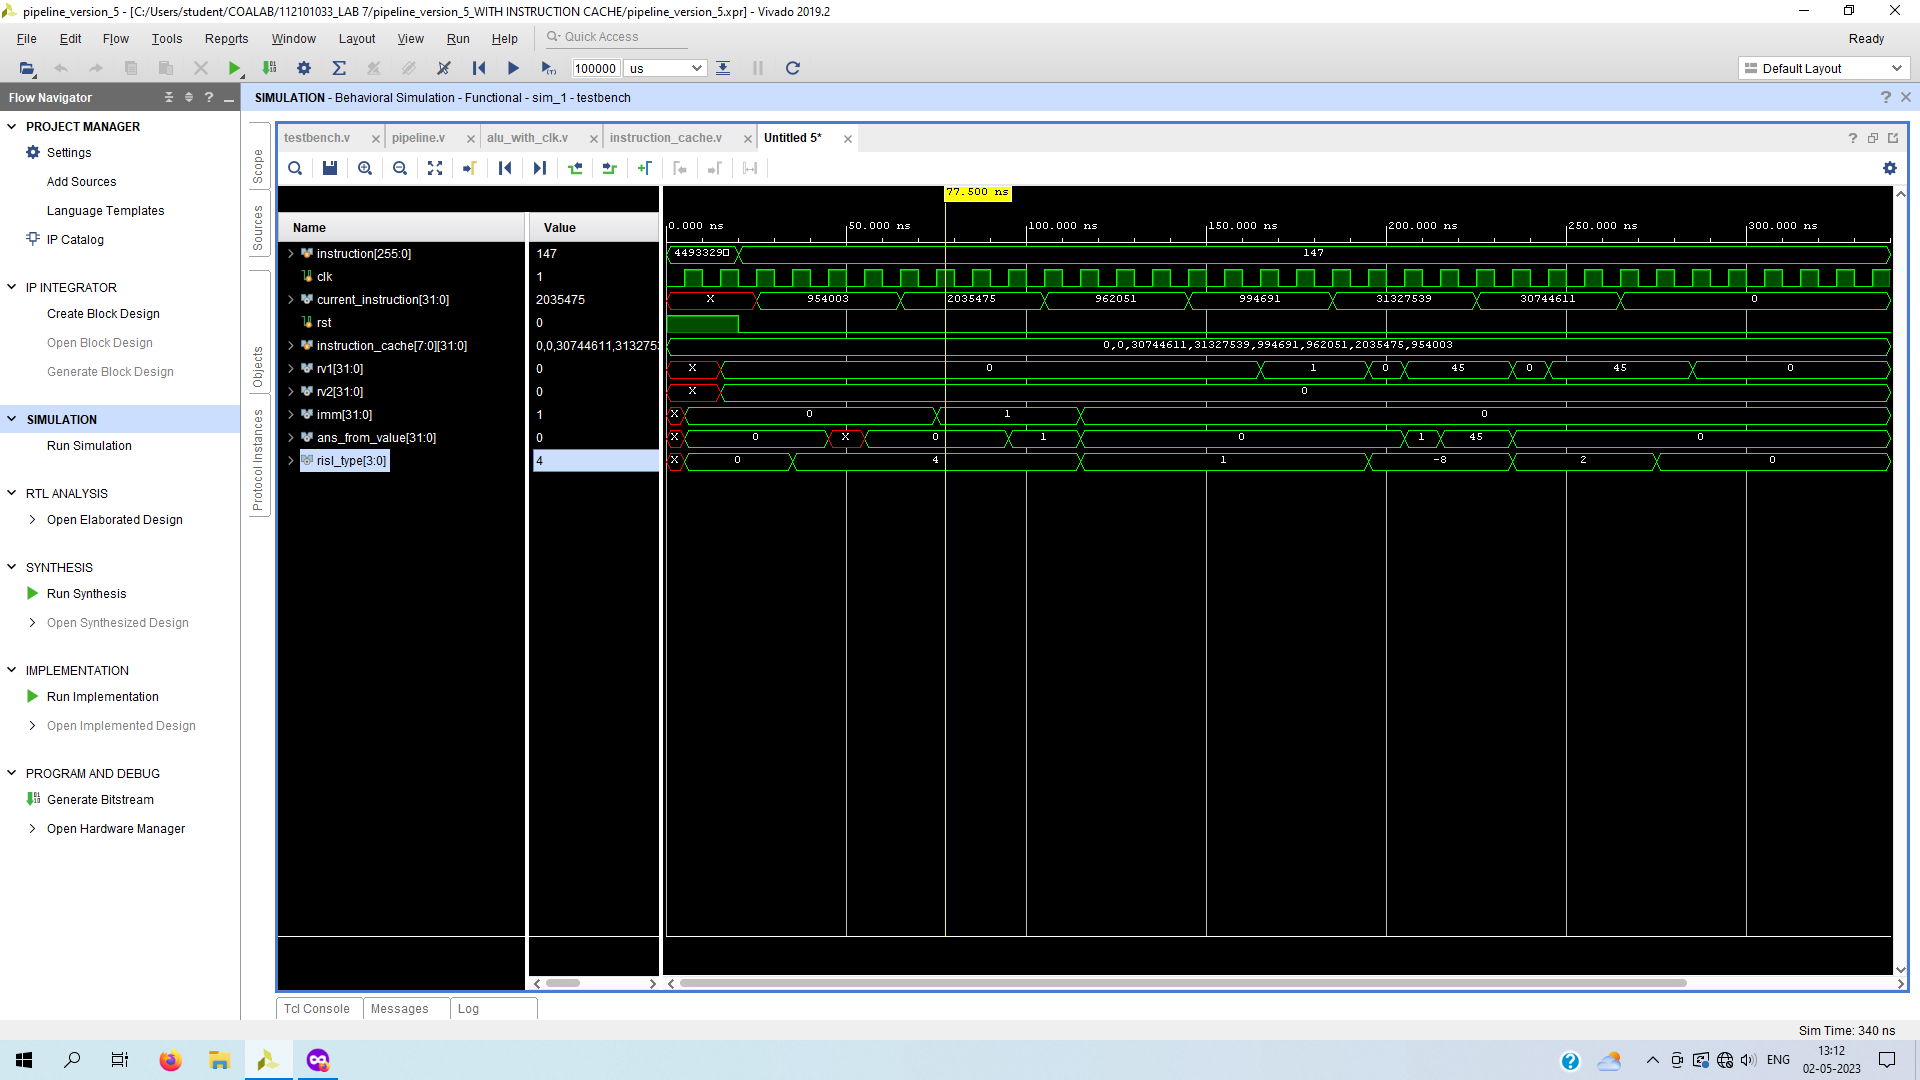
\includegraphics[width=\textwidth]{./images/simulation_lab_7.png}
  \caption{Simulation of Testbench}
  \label{simulation_image}
\end{figure}
% \lipsum[1-3]
In the timing diagram, at the first posedge clk after \textbf{rst becomes zero}, the first instruction is fetched as shown by the \textbf{current\textunderscore instruction} in the simulation image$^{\ref{simulation_image}}$ and it completes it in 4 clock cycles, and the subsequent instruction is fetched and this goes on till the program counter reaches the end of the instruction.
\begin{itemize}
  \item The read value 1 is shown as rv1.
  \item The read value 2 is shown as rv2.
  \item The immediate value is shown as imm.
\end{itemize}

% \section{Discussion}
This part is reserved for discussion.


WHAT SHOULD WE WRITE IN THIS DISCUSSION PAGE????????

% \cite{Dummy4}.

% \lipsum[2-5]

\section{Conclusion}
We have developed a complete pipeline in Verilog with instruction cache and data cache.
% \lipsum[1-5]

\section{Contributions}
  The instruction cache and the data cache was done together and there was equal splitting of the work to the team members.
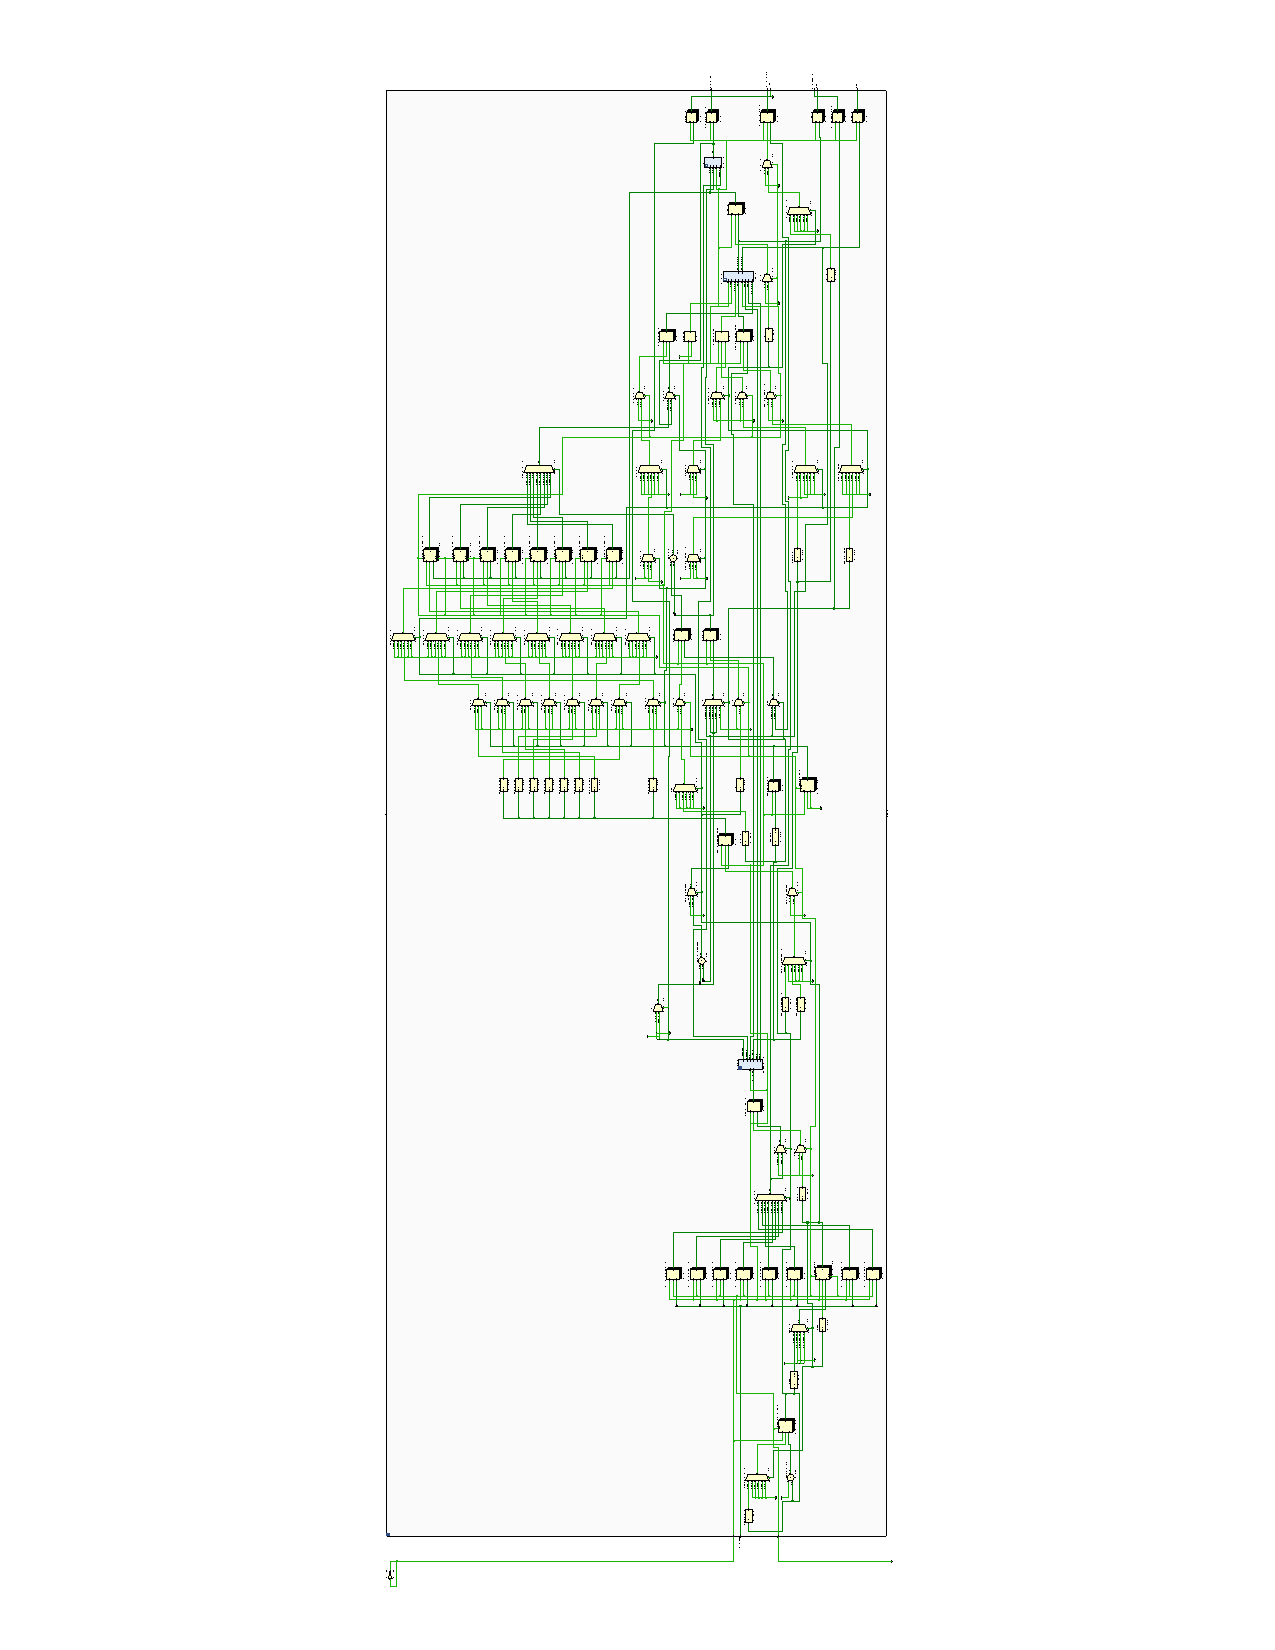
\includepdf[pages={1}]{PIPELINE_LAB_7_SCHEMATIC_LANDSCAPE}\label{schematic}

\section{Code for Lab 7}\label{code_section}
\subsection{Code for the pipeline}
\lstset{language=Verilog}
\begin{lstlisting}
module pipeline(
  input [255:0] instruction,
  input clk, rst,
  output reg [31:0] rv1, rv2, imm, ans_from_alu,current_instruction,
  output reg [3:0] risl_type_register
  );
  reg [31:0] pipeline_1;
  reg [31:0] pipeline_2 [2:0];
  reg [31:0] pipeline_3 [1:0];
  wire [16:0] opcode_wire;
  wire [4:0] rs1_wire, rs2_wire, rd_wire;
  reg [4:0] destination_register;
  wire [11:0] immediate_wire;
  wire [3:0] risl_type_wire;    
  
  parameter [3:0]
  R_type = 4'b1000,
  I_type = 4'b0100,
  S_type = 4'b0010,
  L_type = 4'b0001;
  reg [31:0] data_cache [7:0];

  decoder_with_clk DECODER(
    pipeline_1,clk,  opcode_wire, rs1_wire, 
    rs2_wire, rd_wire, immediate_wire, risl_type_wire
  );
  
  reg [4:0] rs1, rs2, rd;
  reg enable_write, enable;
  reg [31:0] write_value;
  wire [31:0] read_value_1_wire, read_value_2_wire;
  always @ (posedge clk)
  begin 
  enable <= 1'b1;
  end
  

  reg_file REGISTER_FILE(
    rs1_wire, rs2_wire, destination_register , 
    enable_write, write_value, clk, rst, enable, 
    read_value_1_wire, read_value_2_wire);

  
  reg [31:0] A, B;
  wire [31:0] UH_wire, LH_wire;
  wire overflow;
  reg [4:0] data_cache_address;
  
  
  alu_with_clk ALU(A, B, opcode_wire, clk, UH_wire, LH_wire, overflow_wire);
  
//    always @
//    reg store_instruction;
//    reg load_instruction;
  reg [1:0] load_store;
  
  
  parameter [2:0]
  STAGE_1 = 3'd1,
  STAGE_2 = 3'd2,
  STAGE_3 = 3'd3,
  STAGE_4 = 3'd4;
  
  reg [2:0] stage;
  
  always @ (posedge clk) begin
      rv1 <= read_value_1_wire;
      rv2 <= read_value_2_wire;
      imm <= immediate_wire;
      ans_from_alu <= LH_wire;
      risl_type_register <= risl_type_wire;
  end
  
  always @ (posedge clk) begin
      case(risl_type_wire)
      S_type: load_store = 2'b01;
      L_type: load_store = 2'b10;
      default: load_store = 2'b00;
      endcase
  end
  
  reg [31:0] instruction_cache [7:0];
  reg [3:0] program_counter;

  reg [31:0] temp;
  integer i;
  always @ (posedge clk) begin
      if (rst) begin
          stage = 3'd1;
          for (i=0;i<8;i=i+1) data_cache[i] = 32'h0; 
          load_store = 2'b0;
          data_cache[0] = 45;
          data_cache[1] = -20;
          program_counter = 4'b0;
          for (i=0;i<8;i = i + 1) instruction_cache[i] = 32'h0;
          instruction_cache[0] = instruction[31:0];
          instruction_cache[1] = instruction[63:32];
          instruction_cache[2] = instruction[95:64];
          instruction_cache[3] = instruction[127:96];
          instruction_cache[4] = instruction[159:128];
          instruction_cache[5] = instruction[191:160];
          instruction_cache[6] = instruction[223:192];
          instruction_cache[7] = instruction[255:224];
// for(i=0; i<8; i=i+1) 
//  begin
//  $display("INSTRUCTION FROM PIPELINE IS ", instruction_cache[i]);
//  end
      
      end
      else begin
      
          case(stage)
              STAGE_1: begin
                  if(program_counter == 9) begin
                      stage = STAGE_1;
                      pipeline_1 = 32'h0;
                  end
              
              else begin
              
//                    pipeline_1 = instruction[31: 0];
                  pipeline_1 = instruction_cache[program_counter];
                  current_instruction = pipeline_1;
                  program_counter = program_counter + 1;
                  enable_write = 1'b0;
//                    pipeline_1 = instruction;
                  data_cache_address = 5'h0;
                  $display("instruction is ",pipeline_1);
  //                $display("first cycle");
                  stage = STAGE_2;
              end
              
              
              end
              STAGE_2: begin
              // waiting for output from decoder
//                $display("second cycle");

              stage = STAGE_3;
//                $display("A and B are    ",A, B);
              
              end
              STAGE_3: begin
              A = read_value_1_wire;
//                $display(" A is ", A);
//                B = read_value_2_wire;
              case(risl_type_wire)
                  R_type: 
                  begin
                  B = read_value_2_wire;
                  destination_register = rd_wire;
                  end
                  I_type: begin
                  
                          destination_register = rd_wire;
                          if (~immediate_wire[11]) B = {20'b0, immediate_wire};
                          else B = {20'hfffff, immediate_wire};
                          
                  end
                  S_type:begin
                  
                      destination_register = rd_wire;
                      temp = read_value_2_wire;
                      
                      
                      if (~immediate_wire[11]) B = {20'b0, immediate_wire};
                          else B = {20'hfffff, immediate_wire};
//                        $display(" A and B for store instruction are ", A, B);
//                        $display("rv1 is ", read_value_1_wire);
                      
                      
                      data_cache_address = B + temp;
//                        $display("dca is ..........",data_cache_address);
                  
                  end
                  L_type:
                  begin
                      temp = read_value_1_wire;
                      if (~immediate_wire[11]) B = {20'b0, immediate_wire};
                          else B = {20'hfffff, immediate_wire};
                      
                  
                  end
                  
                  
                  default: 
                  begin
                  B = 32'b0;
                  destination_register = rd_wire;
                  
                  end
                  
                  
                  
              endcase
//                $display("A and B are    ",A, B);
                  stage = STAGE_4;
//                    enable_write = 1'b1;
//                    write_value = LH_wire;
////                    $display("lh wire in third cycle is ", LH_wire);
////                    $display("write value is ",write_value);
//                    stage = STAGE_1;
              
              
              end
              STAGE_4: begin
//                $display("LH wire in 4th cycle is ",LH_wire);
//                            enable_write = 1'b1;

//                    write_value = LH_wire;
//                    $display("lh wire in third cycle is ", LH_wire);
//                    $display("write value is ",write_value);
                  
                  
                  case(load_store)
                      2'b10:begin
                      // load instruction
                      enable_write = 1'b1;
// lh wire from alu is the address from where we 
//have to take the value from data cache and place it in destination register
                      destination_register = rd_wire;
                      write_value = data_cache[temp+B];
                      $display("write value is ", write_value);
                      
                      
                      end
                      2'b01:
                      begin
                      //store instruction
//                        enable_write = 1'b1;
                      enable_write = 1'b0;
//                        write_value
// address is in lh wire, we have to write the 
// read data from register file to data cache[lh wire]
                      data_cache[data_cache_address] = A;                        
                      
                      end
                      default:
                      begin
                          enable_write = 1'b1;
                          write_value = LH_wire;
                          
                      
                      end
                      
                      
                  endcase
                  stage = STAGE_1;
                for (i=0;i<8;i=i+1) $display("%d value is %b",i, data_cache[i]);
              end
              
              default: begin
              end
          endcase
      end
  end

endmodule
\end{lstlisting}




\subsection{Code for Testbench}
\lstset{language=Verilog}
\begin{lstlisting}
  
module testbench;
reg [255:0] instruction;
reg clk, rst;
reg [31:0] instruction_cache [7:0];
// the above is the instruction cache which holds the instruction




wire [31:0] rv1, rv2, imm, ans_from_value,current_instruction;
wire [3:0] risl_type;

pipeline DUT(
  instruction, clk, rst, rv1, rv2, imm, 
  ans_from_value,current_instruction,risl_type
);
// the instruction passed to the pipeline 
// module is a single string of 8*32 = 256 bits


initial begin
clk = 1'b0;
rst = 1'b1;
instruction_cache[0] = {12'd0,5'd29,3'b000,5'd29,7'b0010011};
instruction_cache[1] = {12'd1,5'd30,3'b000,5'd30,7'b0010011};
instruction_cache[2] = {12'd0,5'd29, 3'b010, 5'd28, 7'b0000011};
instruction_cache[3] = {12'd0,5'd30, 3'b010, 5'd27, 7'b0000011};
instruction_cache[4] = {7'b0, 5'd29, 5'd28, 3'b0, 5'd10, 7'b0110011};
instruction_cache[5] = {7'b0,5'd29,5'd10, 3'b010, 5'd0, 7'b0100011};
instruction_cache[6] = 32'h0;
instruction_cache[7] = 32'h0;
instruction = {instruction_cache[7],instruction_cache[6],instruction_cache[5],instruction_cache[4],instruction_cache[3],instruction_cache[2],instruction_cache[1],instruction_cache[0]};
// instruction = {
//     instruction_cache[7],instruction_cache[6],
//     instruction_cache[5],instruction_cache[4],
//     instruction_cache[3],instruction_cache[2],
//     instruction_cache[1],instruction_cache[0]
// };

#20
rst = 1'b0;
//    $display("instruction from testbench is ", instruction);






#320 $finish;

end

always #5 clk = ~clk;

endmodule


\end{lstlisting}

% % \pagebreak
% \nocite{*}
% \bibliographystyle{ieeetr}
% \bibliography{library}

\end{document}